% Appendix A

\chapter{Enquêtes \& interviews}\label{ch:Enquetes-interviews}
\section{Enquêtes}\label{sec:enquetes}

Om inzicht te verkrijgen in de belangen van de verschillende stakeholders is een enquête uitgezet naar de interne stakeholders van Eaglescience over SOUP-analyses. De enquête bestond uit 5 vragen en was verzonden naar 15 medewerkers en de response rate was 100\%. Hieronder worden de uikomsten van de enquête besproken.\\

\textbf{Vraag 1: Wat is jouw functie binnen Eaglescience?}\\
\begin{figure}[bth]
    \centering
    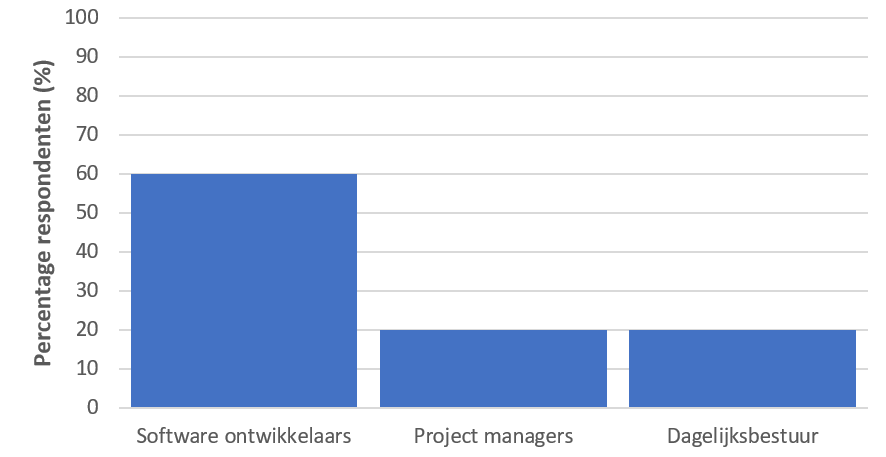
\includegraphics[width=8cm]{gfx/appendix/Vraag1}
    \caption{functies binnen Eaglescience}
    \label{fig:enqueteV1}
\end{figure}

Het leeuwendeel van de respondenten bekleed de functie software ontwikkelaar, terwijl 20\% project managers zijn, en 20\% onder het dagelijks bestuur valt (figuur ~\ref{fig:EnqueteV1}).\\

\textbf{Vraag 2: Voer jij zelf SOUP-analyses uit?}\\
\begin{figure}[bth]
    \centering
    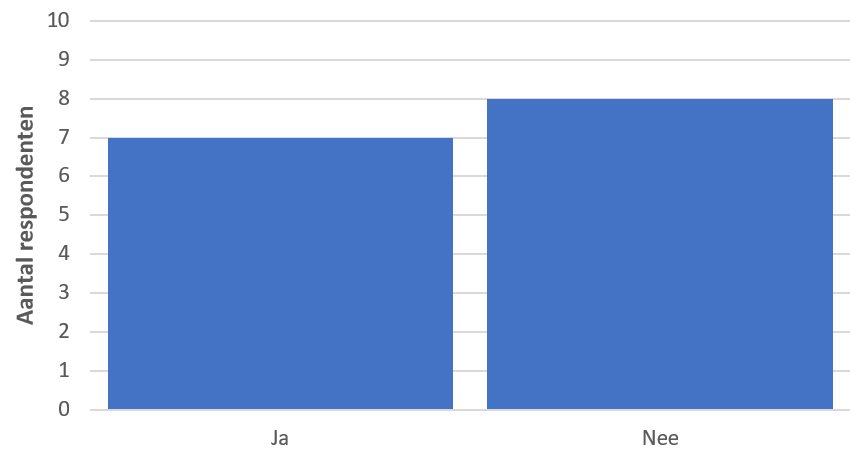
\includegraphics[width=8cm]{gfx/appendix/Vraag2}
    \caption{Voer jij zelf SOUP-analyses uit?}
    \label{fig:EnqueteV2}
\end{figure}
Enkel Software ontwikkelaars binnen Eaglescience voeren zelf SOUP-analyses uit, terwijl de overige respondenten dit niet doen. Van de software ontwikkelaars is er een kleine groep die niet zelf betrokken is bij de SOUP-analyses (figuur ~\ref{fig:EnqueteV2}).\\

\textbf{Vraag 3: (indien van toepassing) Hoevaak doe je een SOUP-analyse per project en hoeveel tijd schat je hiermee op jaarbasis kwijt te zijn?}\\
\begin{figure}[bth]
    \centering
    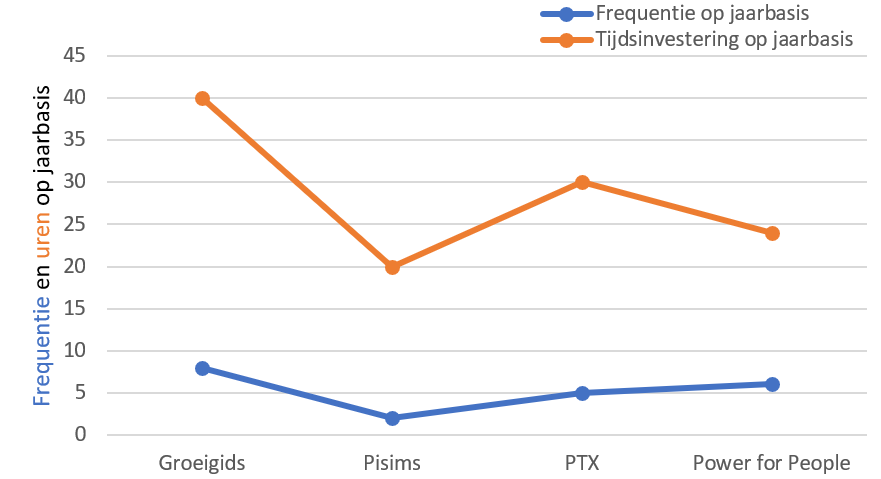
\includegraphics[width=8cm]{gfx/appendix/Vraag3}
    \caption{Hoeveel tijd wordt er besteed aan SOUP-analyses}
    \label{fig:EnqueteV3}
\end{figure}

Voor de uitwerking van deze vraag is de totale frequentie en hoeveelheid    uren die door de individuele respondenten is ingevuld opgeteld. De grafiek weerspiegeld daarom de totale tijdsinvestering binnen Eaglescience aan SOUP-analyses. Gemiddeld wordt eens per 2 maanden een SOUP-analyse uitgevoerd. De totale werklast op jaarbasis hiervan is $\pm$114 uur (figuur ~\ref{fig:EnqueteV3}).\\

\textbf{Vraag 4: Hoe groot acht je het belang van SOUP-analyses?}\\
\begin{figure}[bth]
    \centering
    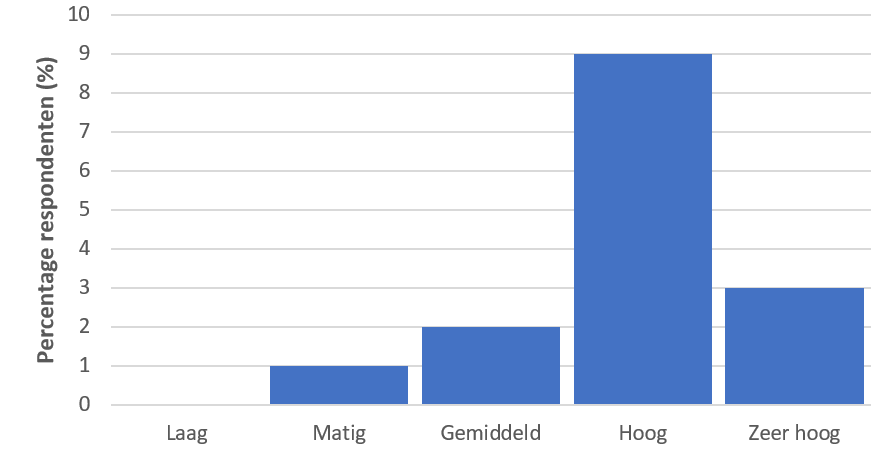
\includegraphics[width=8cm]{gfx/appendix/Vraag4}
    \caption{Het belang van SOUP-analyse}
    \label{fig:EnqueteV4}
\end{figure}
Het leeuwendeel van de respondenten gaf aan een groot belang te hechten aan de data verkregen uit SOUP-analyses (figuur ~\ref{fig:EnqueteV4}).\\

\textbf{Vraag 5: Worden de uikomsten van SOUP-analyses betrouwbaarder wanneer deze automatische in plaats van handmatig worden uitgevoerd?}\\

\begin{figure}[bth]
    \centering
    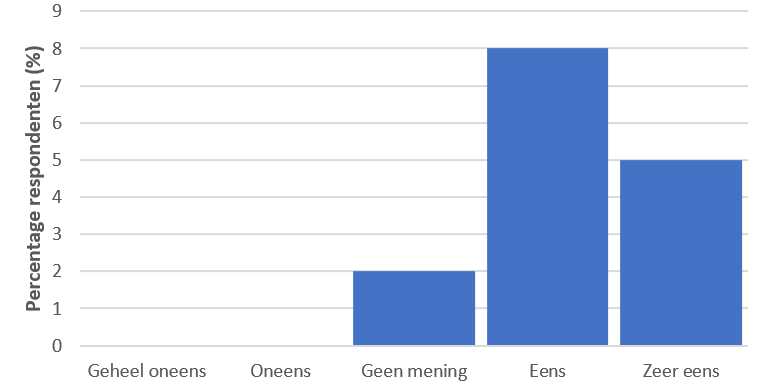
\includegraphics[width=8cm]{gfx/appendix/Vraag5}
    \caption{Betrouwbaarheid van automatisch gegenereerde SOUP-analyse resultaten }
    \label{fig:EnqueteV5}
\end{figure}

De repondenten waren het bijna unaniem eens dat het automatisch uitvoeren van SOUP analyses betrouwbaardere resultaten geeft dan wanneer dit handmatig wordt gedaan (figuur ~\ref{fig:EnqueteV5}).

\clearpage
\section{Interviews}\label{sec:interviews}

\subsection{Ontwikkelaar}\label{subsec:ontwikkelaar}
Dit gesprek heeft als doel om te achterhalen welke taken er op dit moment worden uitgevoerd op het gebied van SOUP-analyses en hoeveel tijd hierin wordt geïnvesteerd. Daarnaast is er gevraagd welke verbeteringen er vanuit zijn/haar rol zijn. Dit gesprek heeft plaatsgevonden op 21-10-2021 met Bas Bro.\smallskip

\textbf{Introductie }
Aangegeven dat het gesprek vertrouwelijk is, en dat de tekst hierover ge-edit mag worden door de geïnterviewde.
Daarnaast is er gesproken over zijn functie binnen Eaglescience.
De volgende vragen zijn tijdens het interview gesteld:
\\
\textbf{Welke stappen worden er op dit moment genomen om er zo zeker mogelijk van te zijn dat er geen kwetsbaarheden zitten in de code? }
Voordat een bibliotheek/framework wordt gebruikt wordt de documentatie doorgenomen en in de repositories nagegaan hoe actief en hoe vaak er gebruik van gemaakt wordt. Hoe actiever en vaker een bibliotheek gebruikt wordt hoe groter de kans dat er bugs en dergelijke worden ontdekt wat weer de kans kleiner maakt op kwetsbaarheden. Op het moment dat een bibliotheek gebruikt wordt tijdens de ontwikkeling binnen onze projecten wordt er geprobeerd om de versies zo up-to-date mogelijk te houden. Het updaten naar een major wordt tijdens ontwikkeling niet veel gedaan, maar meestal meegenomen in onderhoudssprints.

Op een aantal momenten wordt er handmatig een analyse uitgevoerd waarbij iedere bibliotheek en framework wordt gecontroleerd op kwetsbaarhden in verschillende databases. We maken nu al gebruik van NPM audit voor de Angular projecten. Maar SBT is vaak handwerk. Bij gevonden kwetsbaarheden wordt alles met de hand bijgewerkt.
\\

\textbf{Heb je het idee dat de tijd die nodig is om deze stappen te zetten opweegt tegen het behaalde resultaat? } De manier waarop er nu SOUP-analyses worden uitgevoerd is tijdrovend. Waarbij er nog bovenop komt dat er bij gevonden kwetsbaarheden de software ook geupdate moet worden. Het is veel werk en vaak is het resultaat niet direct te merken door een klant of door collega's wat het klusje niet heel populair maakt. Als de module ervoor kan zorgen dat in ieder geval het zoeken naar bekende kwetsbaarheden uit kan voeren zal dat al schelen in de tijd wat weer in het updaten van de applicatie kan worden gestoken of in verdere ontwikkeling.
\\



\textbf{Wat zou volgens jou een ideale situatie zijn mocht je een module mogen ontwikkelen om de SOUP-analyse automatisch te doen? }Het meest ideaal zou zijn dat er naast een analyse ook een mogelijkheid is om informatie te verkijgen over de eventueel gevonden kwetsbaarheden zodat er makkelijk kan worden besloten of de kwetsbaarheid invloed heeft op de applicatie die wordt ontwikkeld. Naast deze informatie zal een samenvating van alleen kwetsbaarhden met een bepaalde impactgraat (lees: Severe, High, Medium, Low) ook al schelen op het moment dat er snel moet worden aangetoond of een applicatie veilig is.
\\

\textbf{Heb je aanvullingen of opmerkingen op basis van de eerder naar je toegestuurde requirements? } Op de samenvatting, en het geven van extra informatie heb ik geen aanvullingen en opmerkingen.
\\

\subsection{Project manager}\label{subsec:project-manager}
Dit gesprek heeft als \textbf{doel} de informatie behoeften van een projectmanager in kaart te brengen. Dit gesprek heeft plaatsgevonden op 21-10-2021 met Jeroen
\\
\textbf{Introductie }
Aangegeven dat het gesprek vertrouwelijk is en dat het ge\-edit mag worden door de geïnterviewde, als ook welke functie er bekleed wordt door de geïnterviewde.
\\
\textbf{Hoe verkrijg je op dit moment de informatie om beslissingen te nemen om kwetsbaarheden op te lossen? }
De ontwikkelaars houden eens is de zoveel tijd een SOUP-analyse op de gebruikte bibliotheken. Op basis van deze analyse wordt gekeken welke impact een kwetsbaarheid kan hebben als deze gevonden is, waarop vervolgens wordt ingeschat welke prioriteit het is en hoeveel effort het kost om te fixen.
\\
\textbf{Zou het volgens jou verschil uitmaken dat er automatisch een analyse wordt uitgevoerd ten opzichte van de kwaliteit van de software? }Zoals gezegd wordt eens in de zoveel tijd een analyse gehouden. Ik denk dat een geautomatiseerde manier van kwetsbaarheden opsporen een kans biedt om de analyses vaker uit te voeren met daarbij de mogelijkheid dat de software veiliger wordt. Al moeten de updates wel uitgevoerd blijven worden door de ontwikkelaars, maar het feit dat er mogelijk 1 keer per week een analyse uitgevoerd wordt maakt de pak kans op kwetsbaarheden groter. Uiteindelijk zal de ideale situatie zijn dat er ook wordt gegekeken naar mogelijke updates voor bibliotheken die we gebruiken om zo ook op deze manier kwetsbaarheden voor te zijn en een betere inschatting te kunnen maken hoeveel effort het kost om die up-date te doen.
\\

\textbf{Zou dit dan ook ten goede komen met betrekking tot budgetten en dergelijke. Met andere woorden zouden ontwikkelaars meer tijd hebben om te ontwikkelen?} Ik denk het wel. Al zal dat voornamelijk afhangen van de hoeveelheid kwetsbaarheden die gevonden worden.
\\
\textbf{Op welke manieren zou je de informatie willen zien in de portal?} Er bestaat nu een module projecten in de portal. Het zou ideaal zijn om hier een samenvatting te kunnen plaatsen met de mogelijkheid om vervolgens in een eigen module binnen de portal meer gedetaileerde informatie te verkrijgen. Zo kan een project manager sneller een inschatting maken per project en de ontwikkelaar vervolgens de vervolg stappen inzien.
\\
\textbf{Op basis van de getoonde requirements tot nu toe zijn er aanvullingen die direct tot je komen?} Alleen dat het wellicht ook handig is om update informatie van gebruikte bibliotheken inzichtelijk te maken.
